\textbf{COLUNI 2024 -- Questão 21}\par\medskip Leia os textos a seguir.

\textbf{Texto I}

\noindent
\begin{minipage}[t]{0.30\linewidth}
\includegraphics[page=9,trim=66pt 496pt 385pt 169pt,clip,height=6.2cm]{static/simulados/coluni/provas/2024.pdf}
\end{minipage}\hfill
\begin{minipage}[t]{0.66\linewidth}
Chimamanda Ngozi Adichie was born in Enugu, Nigeria in 1977. Her first novel, \textit{Purple Hibiscus} (2003), won the Commonwealth Writers’ Prize, and her second novel, \textit{Half of a Yellow Sun} (2006), won the Orange Prize. Her 2013 novel \textit{Americanah} won the US National Book Critics Circle Award. She was named one of TIME Magazine’s 100 Most Influential People in the World in 2015. In 2017, Fortune Magazine named her one of the World’s 50 Greatest Leaders. She is a member of both the American Academy of Arts and Letters and the American Academy of Arts and Sciences.

(Chimamanda Ngozi Adichie. Chimamanda, 2023. Disponível em: https://www.chimamanda.com/about/. Acesso em: 9 jul 2023. Adaptado).
\end{minipage}

\textbf{Texto II}

\begin{center}\textbf{Chimamanda Ngozi Adichie speaks at a special fundraiser in support of female candidates in elections.}\end{center}

I have often said that I don't think women are inherently better than men. Women are human. So I think it is not that women are better than men, but because of the challenges women face, and because of the socialization women experience, women are more likely to do things differently, and women are more likely to think of consensus. For example, women are more likely to put their ego aside. And so for me, one of the things that I find encouraging about supporting women is because there's a likelihood of women doing things differently and better.

But on the other hand, I do not think that the case for women is that they're better, I think the case for women political candidates and political representation is that women are full citizens, and if we want a more perfect democracy then we should want better representation. You cannot have 50 of the population being so severely underrepresented, and let's also remember that women don't have to be perfect.

It is important for us not to think that the woman has to be perfect, and we also have to think about what happens after a woman is elected. We also have to remember that we cannot judge women too harshly. Very often women are held to much higher standards, and so when they fail in ways that human beings fail, it is often made to seem as though it's catastrophic. This severe judgment is because, in some ways, we expect women to be angels rather than accepting that women are human.

Another crucial point is that women need men. In this specific case, women need men to support women in politics. And you know you cannot change a system that is dominated by a group, one particular group, without some sort of collaboration or participation of the members of that group. We need men, and so my question is “how do we find these men to get them involved?” It's still very much a male-centered world, and we need the good men, and I just have to say that if more women were in real positions of power, insecurity would reduce.

(AFRICA WEB TV. Nigerians think they are better than anyone eles. YouTube, 22 JAN 2023. Disponível em: https://www.youtube.com/watch?v=jn-2x9HuJkI&t=16s. Acesso em: 9 jul 2023. Adaptado).

Considerando as informações apresentadas nos textos I e II, é INCORRETO afirmar que:
\begin{enumerate}
\item A escritora nigeriana Chimamanda Ngozi Adichie aborda sobre a importância de uma maior participação e
        da representação das mulheres na política.
\item Chimamanda enfatiza a necessidade do apoio e da participação masculina, uma vez que o mundo
        continua centralizado nos homens.
\item Para a renomada escritora, mulheres são melhores do que os homens em consequência dos desafios que
        enfrentam e da socialização que experienciam.
\item Chimamanda argumenta que mulheres não devem ser julgadas de forma severa e segundo altos padrões
        de referência, como geralmente acontece.
\end{enumerate}
